\documentclass{beamer}
\mode<presentation>
\usetheme{CambridgeUS}
\usepackage[russian]{babel}
\usepackage[utf8]{inputenc}
\usepackage[T2A]{fontenc}
\usepackage{sansmathaccent}

\usepackage{verbatim}
\usepackage{alltt}

\pdfmapfile{+sansmathaccent.map}
\title[Software Design]{Обработка ошибок}
\author{Наумов Д.А., доц. каф. КТ}
\date[21.10.2019] {Основы программной инженерии, 2019}

\begin{document}

%ТИТУЛЬНЫЙ СЛАЙД
\begin{frame}
  \titlepage
\end{frame}
  
%СОДЕРЖАНИЕ ЛЕКЦИИ
\begin{frame}
  \frametitle{Содержание лекции}
  \tableofcontents  
\end{frame}

\section{Обработка ошибок на основе механизма исключений}

\subsection{Варианты обработки ошибок, не связанных с исключениями}

\begin{frame}{Обработка ошибок}
Процесс обработки ошибки можно представить в виде последовательности, состоящей из трех действий:
\begin{enumerate}
\item Выявление ошибочной ситуации. Этап связан с особенностями предметной области и вытекающими из этих особенностей требованиям к данным и организации вычислительного процесса.
\item Генерация информации о возникновении ошибочной ситуации.
\item Обработка ошибки (определение действий в связи с выявленной ситуацией).
\end{enumerate}
Основная сложность \textbf{не в том, как обнаружить ошибку}, а в том:
\begin{itemize}
\item как сообщить об этой ошибке отдельным модулям проекта;
\item как определить набор действий, обрабатывающих ошибочную ситуацию в том случае, когда эта обработка не может быть осуществлена в пределах одной функции и даже в пределах отдельного модуля.
\end{itemize}
\end{frame}

\begin{frame}{Обработка ошибок}
Варианты обработки ошибок:
\begin{itemize}
\item Обработка ошибки на месте.
\item Использование возвращаемых значений.
\item Использование глобальных переменных или переменных-членов класса, исполняющих роль индикаторов состояния приложения или объекта.
\item Использование специально разработанных функций.
\item Использование функций обратного вызова (callback functions).
\item Использование генерации и обработки исключений.
\end{itemize}
\end{frame}

\begin{frame}[fragile]{Обработка ошибок на месте}
\begin{alltt}
procedure QueueInt.Enqueue(Elem: integer); //Записать элемент
begin
  if length = size then begin
    write('Enqueue error. Queue is full.');
    exit;
  end;
  last := (last+1) mod size;
  inc(length);
  body[last] := Elem;
end;
\end{alltt}
\end{frame}

\begin{frame}[fragile]{Обработка ошибок на месте}
Недостатки: 
\begin{itemize}
\item находясь в пределах области видимости функции, где была диагностирована ошибочная ситуация, мы можем не иметь доступа к данным и функциям, необходимым для корректной и полной обработки возникшей ситуации.
\item трудность реализации обработки ошибок разного типа (например, ошибок,
требующих или не требующих остановки выполнения программы).
\end{itemize}
Обработка ошибок на месте затрудняет разработку унифицированных компонентов, которые могли бы использоваться в различных приложениях.
\end{frame}

\begin{frame}[fragile]
\begin{alltt}
//Использование возвращаемого значения
const READ_OK = 0;
      ERROR_UNEXP_EOF = 1;
      ERROR_BAD_FORMAT = 2;
//функция чтения
procedure ReadData(var F: Text; var X: integer; var ErrorCode: integer);
begin
  if EOF(F) then begin
    ErrorCode := ERROR_UNEXP_EOF;
    exit;
  end;
  \{\$I-\} read(F, X);  \{\$I+\}
  if IOResult <> 0 then begin
    ErrorCode := ERROR_BAD_FORMAT;
    exit;
  end;
  ErrorCode := READ_OK;
end; 
\end{alltt}
\end{frame}

\begin{frame}[fragile]
\begin{alltt}
  ReadData(InputFile, InputData, ErrorCode);
  case ErrorCode of
    ERROR_UNEXP_EOF: //обработка ошибки - EOF
      begin
        writeln('Error  - end of file ', FileName);
        halt(2);
      end;
    ERROR_BAD_FORMAT: //обработка ошибки - неверные данные
      begin
        writeln('Error  - bad format in', FileName);
        halt(3);
      end;
  end;
  writeln('X = ', InputData);
  writeln('Terminated succesfully');
\end{alltt}
\end{frame}

\begin{frame}{Возвращаемые значения как инструмент обработки ошибок}
\begin{figure}[h]
\centering
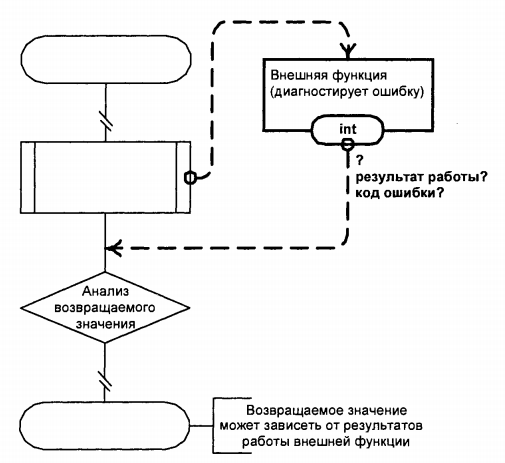
\includegraphics[scale=0.5]{images/lec08-pic01.png}
\end{figure}
\end{frame}

\begin{frame}{Возвращаемые значения как инструмент обработки ошибок}
Недостатки: 
\begin{itemize}
\item + использование возвращаемого значения позволяет отделить реализацию выявления ошибки от обработчика ошибки; 
\item - усложняется интерфейс функций, в которых диагностируется ошибка;
\item - некоторые функции могут использовать возвращаемое значение для реализации элементов решения, не связанных с обработкой ошибок; 
\item - некоторые функции могут заканчиваться с разными кодами ошибок;
\item - в ОО-программах невозможно сообщить об ошибке в ходе выполнения конструктора или деструктора, которые вообще не имеет возвращаемого значения.
\end{itemize}
\end{frame}

\begin{frame}{Использование глобальных переменных}
\begin{itemize}
\item функциональные модули взаимодействуют посредством использования разделяемого ресурса;
\item в случае обнаружения ошибочной ситуации данной переменной присваивается определенное кодовое значение, которое может быть проанализировано за пределами функции, диагностировавшей ошибку;
\item вместо возвращаемого значения используется обособленный интерфейс для взаимодействия функций в связи с обработкой ошибок.
\end{itemize}
\begin{figure}[h]
\centering
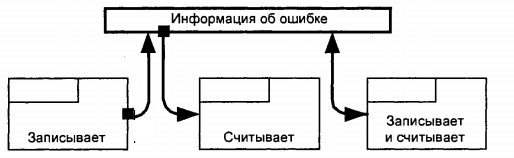
\includegraphics[scale=0.5]{images/lec08-pic02.png}
\end{figure}
\end{frame}

\begin{frame}[fragile]
\begin{alltt}
const
  ErrorCode: integer = NONE;  //код ошибки, начальное состояние NONE

//функция чтения из текстового файла
procedure ReadData(var F: Text; var X: integer);
begin
  if EOF(F) then begin
    ErrorCode := ERROR_UNEXP_EOF;
    exit;
  end;
  \{\$I-\} read(F, X); \{\$I+\}
  if IOResult <> 0 then begin
    ErrorCode := ERROR_BAD_FORMAT;
    exit;
  end;
  ErrorCode := READ_OK;
end;
\end{alltt}
\end{frame}

\begin{frame}[fragile]
\begin{alltt}
  ReadData(InputFile, InputData);
  case ErrorCode of
    ERROR_UNEXP_EOF: //обработка ошибки - EOF
      begin
        writeln('Error  - end of file ', FileName);
        halt(2);
      end;
    ERROR_BAD_FORMAT: //обработка ошибки - неверные данные
      begin
        writeln('Error  - bad format in', FileName);
        halt(3);
      end;
  end;
  ErrorCode := PASSED; 
\end{alltt}
\end{frame}

\begin{frame}[fragile]
\begin{alltt}
const READ\_OK             = 0;
      ERROR\_UNEXP\_EOF     = 1;
      ERROR\_BAD\_FORMAT    = 2;
      ERROR\_READ\_FAILED   = 4;
      ERROR\_WRITE\_FAILED  = 8;
  ErrorState: integer = 0; 
\end{alltt}
Установка кода ошибки чтения в связи с некорректным форматом данных:
\begin{alltt}
  if IOResult <> 0 then begin
    ErrorCode := ERROR\_BAD\_FORMAT or ERROR\_READ\_FAILED;
    exit;
  end; 
\end{alltt}
Функция проверки ошибки чтения:
\begin{alltt}
function IsBadFormat(): boolean;
begin
  Result := ErrorState and ERROR\_BAD\_FORMAT;
end; 
\end{alltt}
\end{frame}

\begin{frame}
\begin{figure}[h]
\centering
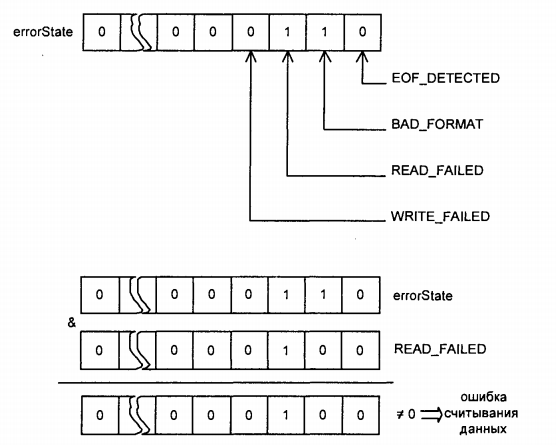
\includegraphics[scale=0.6]{images/lec08-pic03.png}
\end{figure}
\end{frame}

\begin{frame}{Использование специально разработанных функций}
При возникновении ошибочной ситуации функция, диагностировавшая эту ситуацию, просто вызывает подходящую функцию-обработчик, передавая ей код ошибки. 

\begin{itemize}
\item + коды ошибок обычно глобальны на уровне проекта и должны тщательно документироваться. 
\item + обычно реализуется отдельный модуль обработчика ошибок;
\item - не очень подходит для реализации многоуровневых систем обработки ошибок;
\item - подход не всегда может обеспечить универсальный характер обработки ошибочных ситуаций.
\end{itemize}
\end{frame}

\begin{frame}{Использование специально разработанных функций}
\begin{figure}[h]
\centering
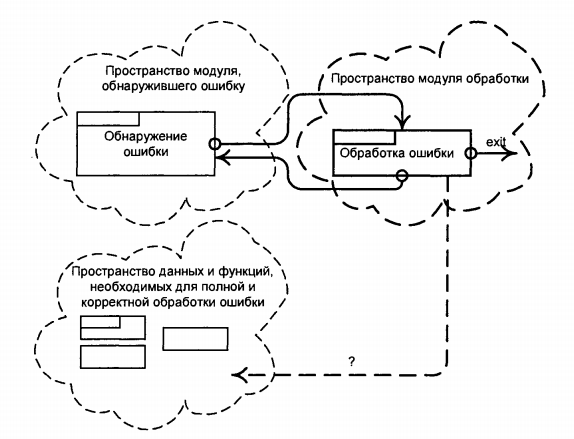
\includegraphics[scale=0.6]{images/lec08-pic04.png}
\end{figure}
\end{frame}

\begin{frame}[fragile]{Использование функции обратного вызова}
Пользователь функции-обработчика ошибок в этом случае должен сначала зарегистрировать функцию обратного вызова, определенную в том модуле, в котором имеется доступ к данным, необходимым для корректной и полной обработки возникшей ситуации. 
\begin{alltt}
type
  TCallbackProc = procedure;
  TErrors = array[0..4] of string;
const
  ERROR_MSG: TErrors = (
    '',
    'Error while opening input file',
    'Error while opening output file',
    'Input file contains no data',
    'Wrong input data format');   
\end{alltt}
\end{frame}

\begin{frame}[fragile]{Использование функции обратного вызова}
\begin{alltt}
procedure Error(ErrorCode: integer; CallbackProc: TCallbackProc);
begin
  writeln('Error No', ErrorCode, ' ', ERROR_MSG[ErrorCode]);
  if CallbackProc = nil then
    halt(0)
  else
    CallbackProc();   //Вызов внешнего обработчика
end;
// Реализация первого варианта завершения программы
procedure Terminatel();
begin
  writeln('Unexpected end of input file');
  writeln('Terminated with error');
  Close(InputFile);
  halt(1);
end;
\end{alltt}
\end{frame}

\begin{frame}[fragile]{Использование функции обратного вызова}
\begin{alltt}
  if IOResult <> 0 then
    Error(2, @Terminate0);

  ReadData(InputFile, InputData);

  if IsEOF then
    Error(3, @Terminatel)
  else if IsBadFormat() then
    Error(4, @Terminate2);
    
  writeln('X = ', InputData);
  writeln('Terminated succesfully');

  Close(InputFile);
  Error(0, nil);    
\end{alltt}
\end{frame}

\begin{frame}{Использование функций обратного вызова}
\begin{figure}[h]
\centering
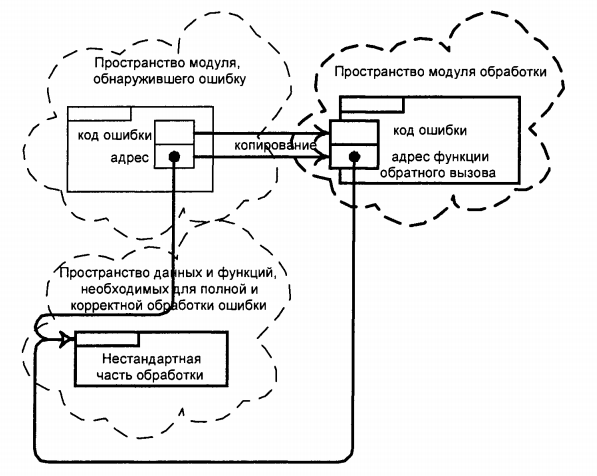
\includegraphics[scale=0.6]{images/lec08-pic05.png}
\end{figure}
\end{frame}

\begin{frame}{Использование функций обратного вызова}
\begin{itemize}
\item + механизм с использованием функций обратного вызова частично разрешает проблему <<разграничения полномочий>> при обработке ошибок;
\item - сигнатура функций обратного вызова должна в точности соответствовать сигнатуре, объявленной в модуле обработки ошибок;
\item - механизм не может считаться полноценной реализацией многоуровневой модели.
\end{itemize}
\end{frame}

\subsection{Обработка исключений}

\begin{frame}{Исключения}
\begin{block}{Исключительная ситуация }
возникает при ошибке или прерывании нормального хода выполнения программы каким-либо событием.
\end{block}
\begin{itemize}
\item Исключение передает контроль выполнения программы обработчику исключительной ситуации, который позволяет отделить нормальную логику работы программы от обработки ошибок. 
\item Поскольку исключения являются объектами, они могут быть сгруппированы в иерархию, использующую наследование, а новые исключения могут объявляться без изменения уже готового кода. \item Исключение может передавать информацию (например, сообшение об ошибке) из точки возникновения исключительной ситуации к месту ее обработки.
\end{itemize}
\end{frame}

\begin{frame}{Исключения}
Механизм обработки ошибок - механизм, встроенный в язык программирования.
Программисту предоставляются:
\begin{itemize}
\item встроенные типы исключений
\begin{itemize}
\item исключения, вызываемые переполнением при выполнении арифметических
операций, 
\item исключения, вызываемые выходом индекса массива за пределы
корректного диапазона) и т.д.
\end{itemize} 
\item возможности для определения собственных исключительных ситуаций.
\end{itemize}
Впервые поддержка обработки исключений средствами языка была реализована в языке PL/1
\end{frame}

\begin{frame}{Основная идея подхода}
\begin{figure}[h]
\centering
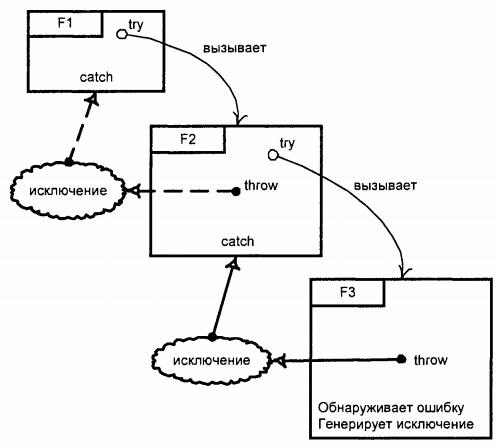
\includegraphics[scale=0.6]{images/lec08-pic06.png}
\end{figure}
\end{frame}

\begin{frame}{Основная идея подхода}
\begin{itemize}
\item Пусть функция F2() в иерархии вызовов передает управление другой функции F3(). 
\item В ходе работы функции F3() выявляется некоторая ошибочная ситуация (т. е. функция F3() обнаруживает ошибку). 
\item Функция, обнаружившая ошибку, генерирует (throws, raise) специальный объект, описывающий возникшую исключительную ситуацию (F3 создает объект-исключение). 
\item Выполнение функции, обнаружившей ошибку, прекращается, и управление передается в вызвавшую ее функцию (F2) для реализации действий по преодолению возникшей проблемы (F2 перехватывает (catches) исключение. 
\item Обработкой исключения может заниматься как функция, непосредственно вызвавшая функцию-генератор исключения, так и предшествующие в иерархии вызовов функции (например, F1()).
\end{itemize}
\end{frame}

\begin{frame}[fragile]{Исключение}
Генерация исключения представляет собой создание объекта-исключения. Объект характеризуется типом, например:
\begin{alltt}
\{\$mode objfpc\} //разрешаем использовать объекты Free Pascal
uses
  SysUtils;		  //подключаем модуль, где содержаться описания
  				  //исключений
type
  //описываем свой класс для обработки исключений
  EMyException = class(Exception)
    public
      constructor Create();
  end;
\end{alltt}
\end{frame}

\begin{frame}[fragile]{Исключение}
Для инициирования исключения вам необходимо использовать экземпляр класса исключения с инструкцией raise:
\begin{alltt}
raise ExceptionClass.Create;
\end{alltt}
Синтаксическая форма инструкция инициирования исключения в общем виде имеет следующий вид:
\begin{alltt}
raise [ExceptionObject] [at Address]
\end{alltt}
\begin{itemize}
\item ExceptionObject - экземпляр класса исключения;
\item Address - выражение, которое можно обработать как указатель.
\end{itemize}
\begin{alltt}
raise Exception.Create('Missing parameter') at @MyFunction;
\end{alltt}
\end{frame}

\begin{frame}[fragile]
Блок, обнаруживающий ошибку, инициирует процесс создания объекта исключения:
\begin{alltt}
procedure F3()
begin
  if( /* ошибка... */ ) then
    raise EMyException.Create(); // Генерирует исключение
  // Действия при отсутствии ошибок
end
\end{alltt}
Вызывающая подпрограмма может перехватить исключение и выполнить обработку ошибки:
\begin{alltt}
procedure F2()
begin
  try 
    F3(); // Может генерировать исключение
  except
    on EMyException do ...    // Обработка ошибки
  end;
end;
\end{alltt}
\end{frame}

\begin{frame}[fragile]
Синтаксис инструкции try...except:
\begin{alltt}
try 
  Statements 
except 
  ExceptionBlock 
end
\end{alltt}
\begin{itemize}
\item Statements - группа операторов;
\item ExceptionBlock - блок обработки исключения
\begin{itemize}
\item может быть еще одной последовательностью инструкций;
\item может быть последовательностью обработчиков исключений, разделяемых инструкциями else.
\end{itemize}
\end{itemize}
Обработчик исключения имеет вид:
\begin{alltt}
on Identifier: IdentifierType do Statement
\end{alltt}
\begin{itemize}
\item identifier: необязателен (если присутствует – может быть любым допустимым идентификатором), 
\item IdentifierType – тип для представления исключений, 
\item statement – оператор языка.
\end{itemize}
\end{frame}

\begin{frame}
\begin{figure}[h]
\centering
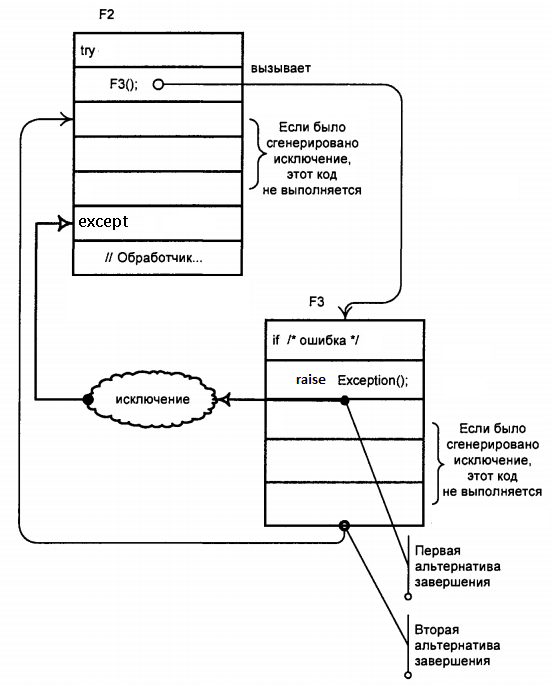
\includegraphics[scale=0.5]{images/lec08-pic07.png}
\end{figure}
\end{frame}

\begin{frame}
\begin{enumerate}
\item Инструкция try...except выполняет команды из изначального списка. Если исключительных ситуаций не возникло, блок исключений игнорируется и управление передается следующей части программы.
\item Если в процессе выполнения списка команд возникла исключительная ситуация (она может быть инициирована инструкцией raise в списке команд или внутри процедуры или функции, вызываемой из этого списка) предпринимается попытка обработки исключительной ситуации:
\item Если какой-либо из обработчиков в exception block подходит для обработки инициированного исключения, управление передается первому такому обработчику. Обработчик подходит для исключения только в том случае, когда тип, указанный в нем, является типом исключения или предком его класса.
\item Если обработчика не найдено, управление передается инструкции в секции else (если таковая присутствует).
\end{enumerate}
\end{frame}

\begin{frame}
\begin{enumerate}
\setcounter{enumi}{4}
\item Если блок обработчиков – это просто последовательность инструкций без каких либо обработчиков – управление передается первой инструкции в этой последовательности.
\item Если ни одно из указанных выше условий не выполнено, поиск продолжается в блоке обработчиков внешней инструкции try...except , выход из которой еще не выполнен. Если и там не находится соответствующего обработчика, секции else или последовательности инструкций, поиск продолжается в следующей внешней инструкции и так далее. Если в самой внешней инструкции исключительная ситуация не будет обработана – приложение завершается.
\end{enumerate}
\end{frame}

\begin{frame}[fragile]
В следующем примере первый обработчик обрабатывает исключение деления на ноль, второй – ошибки переполнения, а последний – остальные математические исключения. SysUtils.EMathError указан последним в блоке обработчиков, так как он является предком обоих этих классов. Если бы он указан первым, последующие обработчики никогда не были бы вызваны:
\begin{alltt}
try
  ...
except
  on EZeroDivide do HandleZeroDivide;
  on EOverflow do HandleOverflow;
  on EMathError do HandleMathError;
end;
\end{alltt}
\end{frame}

\begin{frame}[fragile]
В обработчике исключения перед именем класса исключения можно указать идентификатор. Таким образом объявляется идентификатор для представления объекта исключения в процессе выполнения инструкции, следующей за on...do. Видимость идентификатора ограничивается этой инструкцией. Например:
\begin{alltt}
try
  ...
except
  on E: Exception do ErrorDialog(E.Message, E.HelpContext);
end;
\end{alltt}
\end{frame}

\begin{frame}[fragile]
Если блок исключения имеет секцию else, в этой секции происходит обработка всех исключений, которые не были обработаны в блоке обработчика исключения. То есть:
\begin{alltt}
try
  ...
except
  on EZeroDivide do HandleZeroDivide;
  on EOverflow do HandleOverflow;
  on EMathError do HandleMathError;
else
  HandleAllOthers;
end;
\end{alltt}
В этом примере секция else обрабатывает все исключения, не являющимися SysUtils.EMathError.
\end{frame}

\begin{frame}[fragile]
Блок исключения, не содержащий обработчиков, но содержащий список инструкций, обрабатывает любые исключения. Например:
\begin{alltt}
try
   ...
except
   HandleException;
end;
\end{alltt}
Здесь подпрограмма HandleException обрабатывает все исключенительные ситуации, которые возникают при выполнении инструкций между try и except.
\end{frame}

\begin{frame}[fragile]
\begin{itemize}
\item Если в контексте работы функции F2() исключение не может быть обработано полностью, эта функция может инициировать повторное исключение с тем, чтобы оно было обработано на следующих уровнях иерархии вызовов:
\end{itemize}
\begin{alltt}
procedure F2()
begin
  try 
    F3(); // Может генерировать исключение
  except
    on EMyException do 
      begin 
        // Частичная обработка ошибки
        // ...
        raise;
      end;
  end;
end;
\end{alltt}
\end{frame}

\begin{frame}[fragile]
Код, выполняемый в обработчике исключения может сам инициировать и обрабатывать исключительные ситуации. Поскольку исключения обрабатываются внутри обработчика, они не оказывают влияния на первичное исключение. Тем не менее, если исключение инициированное внутри обработчика, не обрабатывается в нем, первичное исключение теряется.
\begin{alltt}
type
   ETrigError = class(EMathError);
   function Tan(X: Extended): Extended;
   begin
      try
        Result := Sin(X) / Cos(X);
      except
        on EMathError do
        raise ETrigError.Create('Invalid argument to Tan');
      end;
   end;
\end{alltt}
\end{frame}

\begin{frame}[fragile]
Иногда вам необходимо быть уверенными, что некоторые части операции выполнены, вне зависимости от того, прерывается ли выполнение операции исключением или нет. Например, если подпрограмма получает управление ресурсом, важно чтобы память, которую он занимает, была освобождена несмотря на то, что подпрограмма завершается ошибкой. В таких ситуациях вы можете использовать инструкцию try...finally.
\begin{alltt}
Reset(F);
try
   ... // process file F
finally
   CloseFile(F);
end;
\end{alltt}
\end{frame}

\begin{frame}[fragile]
Синтаксис инструкции try...finally выглядит следующим образом:
\begin{alltt}
try statementList1 finally statementList2 end
\end{alltt}
\begin{itemize}
\item Инструкция try...finally выполняет инструкции в statementList1 (секция try). 
\item Если выполнение statementList1 завершается без ошибок, выполняется statementList2 (секция finally). 
\item Если в процессе выполнения statementList1 возникает исключительная ситуация, управление передается в statementList2, когда statementList2 завершает свою работу исключение инициируется повторно. 
\item Если в процессе выполнения statementList1 происходит вызов процедур Exit, Break или Continue – управление выходит из statementList1 , statementList2 выполняется автоматически.
Cекция finally выполняется всегда, вне зависимости от того, как завершается работа секции try.
\item Если в секции finally возникает исключительная ситуация, которая не обрабатывается, исключение выводится из из инструкции try...finally, а исключение, инициированное в секции try, разрушается. 
\end{itemize}
\end{frame}

\begin{frame}{Преимущества встраивания в язык обработки исключительных ситуаций}
\begin{itemize}
\item Без обработки исключений код, необходимый для обнаружения ошибок,
может сильно запутать программу. 
\item Возможность передавать исключительные ситуации для обработки в другие модули.
\item Язык поощряет программиста рассматривать все события, которые могут
возникнуть в процессе выполнения программы, а не игнорировать их в надежде на то, что "ничего плохого не случится".
\end{itemize}
\end{frame}

\begin{frame}[fragile]
\begin{itemize}
\item Предпочтительнее использовать в качестве типов исключений типы, определяемые пользователем
\item В классе исключения можно реализовать часть функциональности в связи с обработкой данного типа исключения, например, получение описания исключительной ситуации.
\end{itemize}
\begin{alltt}
type
  // Тип-исключение "пустой файл"
  EmptyFileException = class(Exception) end;
  // Тип-исключение "ошибка формата данных
  BadFormatException = class(Exception) end;
procedure ReadData(var F: Text; var X: integer);
begin
  if EOF(F) then raise EmptyFileException.Create('EmptyFileException');
  try read(F, X);
  except
    raise EmptyFileException.Create('EmptyFileException');
  end;
end;
\end{alltt}
\end{frame}

\begin{frame}[fragile]
\begin{alltt}
  try
    assign(InputFile, FileName);
    reset(InputFile);
  except
    //обработка ошибки открытия файла
    on EInOutError do
      begin
        writeln('Cannot open file');
        readln;
        halt(1);
      end;
  end;
\end{alltt}
\end{frame}

\begin{frame}[fragile]
\begin{alltt}
  try
    ReadData(InputFile, InputData);
  except
    on EmptyFileException do
      begin
        // Обработка ошибки пустого файла
      end;
    on BadFormatException do
      begin
        // Обработка ошибки формата данных файла
      end;
  end;
\end{alltt}
\end{frame}

%исключения в конструкторах и деструкторах

\end{document}